\section{Implementation}
\label{sec:implementation}

In this section, we introduce some existing implementations of Vivian and some other potential implementations for the planned features.

\subsection{Software \& Dependencies}

The whole project is currently developed in Golang v1.16\footnotetext{Golang website: https://golang.org/}.
And the platform is divided into two parts: the node software, \textit{vivian-node}, and the client software, \textit{vivian-client}.
In the future, there will be another version of the node software, which runs as a plugin of GoHornet, IOTA's node software built in Golang.
The advantage of this version is for direct access to a network instead of connecting to and trust other parties' nodes.

\subsubsection{Node Software} It sets up a node in the peer network layer. These nodes form and help to maintain a decentralized P2P network that let users find naming information.
Each node keeps track of the naming key-value bindings by listening to the live transactions on Tangle DL, filtering naming transactions, parsing transactions, and update related key-value information on the local database.
For listening live transactions, the current implementation subscribes ``tx" (incoming new transactions) and ``sn" (confirmed new transactions) topics of an IOTA node's ZMQ\footnote{ZMQ: ZeroMQ, an asynchronous messaging library for distributed or concurrent applications by providing a message queue.} port.
In the plugin version, the Vivian node is also an IOTA node, so that live transactions can be retrieved from the local database directly.
Besides, the node software is also responsible for handling user requests such as checking whether his/her naming operations are successful and, getting the name binding values, checking the availability of a name, etc.

\subsubsection{Client Software} It provides a user interface (currently CLI) for sending name operation transactions and requests to peer network nodes.
When initializing the client software, it creates an IOTA seed and encrypt it with a password or load a seed from a local encrypted file.
Then users can use the seed to generate public addresses and send transactions for name registration, update, revoke, etc.
The client software can also connect to the nodes in peer network layer, for finding the name binding value, and validating name operations.

\subsubsection{Dependencies} In operating Vivian, we need to do a lot of work related to key-value pairs, and information is stored in \textit{BadgerDB}\footnote{BadgerDB: an embeddable, persistent and fast key-value (KV) database written in pure Go. Github repository: https://github.com/dgraph-io/badger}.
We use libraries in \textit{iota.go}\footnote{iota.go: official Go client library for interacting with the Tangle. Github repository: \url{https://github.com/iotaledger/iota.go}} for handling transactions on Tangle.
We use functions in \textit{go-libp2p}\footnote{go-libp2p: implementation of the libp2p networking stack in Golang. Github repository: \url{https://github.com/libp2p/go-libp2p}} for peer discovery and peer Communication in the P2P network.
Communication messages are serialized by \textit{Protocol Buffers}\footnote{Protocol Buffers (Protobuf):  a method of serializing structured data. Its performance is even better than JSON.} for better performance.

\subsection{Naming Operations}
In this subsection, we introduce how naming operation information is recorded via transactions on Tangle. And taking name registration as an example, for having an overview of how the naming operations are executed.

\subsubsection{Name Operation Transactions} There are two types of transactions in IOTA Tangle: zero-value transaction and value transaction. And currently, we use zero-transaction format for name operation transactions.
Zero-value transactions are barely transactions with value 0 in the \texttt{value} field.
Data of transactions are encoded in trytes\footnote{Tryte: a concept in ternary numeral system similar to byte in binary numeral system. See details on: \url{https://docs.iota.org/docs/getting-started/0.1/introduction/ternary}}.
Each transaction consists of 2,673 tryte-encoded characters. After decoding the trytes, we can obtain a list of data fields of a transaction. The fields related to naming operations are:

\begin{itemize}
    \item \texttt{hash}: 81-tryte string. It is the transaction hash derived from the values of every transaction field and contains part of the proof-of-work. We can use transaction hash to track and validate the information of a transaction.
    \item \texttt{signatureMessageFragment}: 2,187-tryte string. It is a signature or a message, both of which may be fragmented over many transactions in a bundle.
          This field is used for saving the naming operation information and name binding values. 2,187 trytes' size is enough for most of the use cases.
    \item \texttt{attachmentTag}: 27-tryte integer. It is user-defined tag. This field is used for accelerating the filtering of live transactions.
          For fast selection of related transactions, users are required to set the corresponding two-character logogram for each naming operation transaction.
          And nodes in peer network layer can use tryte formats of the logograms for comparison and identifying name operation transactions without parsing \texttt{signatureMessageFragment} (see TABLE~\ref{table:tags}).
    \item \texttt{address}: 81-tryte string. It contains either the sender's or recipient's address. The address is used for justifying the ownership of a name.
    \item \texttt{attachmentTimestamp}: 9-tryte integer. It is Unix epoch (milliseconds since Jan 1, 1970 after proof of work was done). The timestamp is used for counting the time of the operations, e.g. deciding if the current name is expired.
\end{itemize}

Proof-of-work in the previous description is different from the PoW consensus mechanism in Bitcoin blockchain.
Proof-of-work in IOTA is the method for preventing spamming in the network, similar to Hashcash\footnote{Hashcash: a proof-of-work system used to limit email spam and denial-of-service attacks.} in an email system.

\begin{table}[h]
    \centering
    \begin{tabular}{||c c c||}
        \hline
        Operation & Two-Char Value & Tryte Value \\ [0.5ex]
        \hline\hline
        Preorder  & PO             & ZBYB        \\
        Register  & RG             & ACQB        \\
        Renew     & RN             & ACXB        \\
        Update    & UD             & DCNB        \\
        Transfer  & TF             & CCPB        \\
        Revoke    & RV             & ACEC        \\ [1ex]
        \hline
    \end{tabular}
    \caption{Tags for fast name operation identification}
    \label{table:tags}
\end{table}

\subsubsection{Name Registration} For sending each naming operation transaction, the client software needs to generate a new address by the private seed.
To register a name, the user should send name preordering first. In the current implementation, we use Pedersen Commitment \cite{pedersen1991non} for committing the name.
Client software creates and sends a zero-value transaction with tag ``PO" and the message: ``\texttt{PREORDER : \textlangle Hash Commit Value\textrangle}".
After the transaction is successfully sent, the client software will record the name, transaction hash, G, H, R values of Pedersen commitment to BadgerDB.
IOTA nodes will not receive transactions with timestamps more than 10 minutes ago, so in order to prevent front-running, we set the time gap of preorder operation and register operation to be 15 minutes.
After 15 minutes, the user can then send the transaction for name registration. Client software will send a zero-value transaction with tag ``RG", and the message containing the name, G, H, R of Pedersen commitment, preorder transaction hash, and binding value of the name.
Nodes in the peer network layer keep listening to the live transactions on Tangle. If it detects a transaction with tag value in tryte ``ACQB" with appending 9s, it will parse this transaction and check the format of the message.
Then it uses the information provided in the message field to validate name registration. Once the validation is confirmed, it records the name information on its local database and appends this change to the change list.
The change will be broadcast to other nodes in the network via Gossip protocol later.

\subsection{Network}
libp2p network stack provides very powerful functionalities for establishing a distributed network.

\subsubsection{Peer Discovery}
Following procedures are implemented in peer discovery:

\begin{enumerate}
    \item \textbf{Bootstrap.} Nodes will often connect to a bootstrap node through its well-known IP address, to join the network for the first time.
    \item \textbf{mDNS.} Nodes can discover peers under the same local network through multicast DNS.
    \item \textbf{DHT Random Walk.} This process is for finding more peers in the network. First, we make a random node ID in the network, and random walk is a query for finding the peer with that ID.
          We ask the peers we know whether they know the node with target ID or not.
          If they do not know, they will recommend the nodes with closer IDs (logic distance calculated by XOR). We continue this process until no closer node can be found.
\end{enumerate}

\begin{figure}[h]
    \centering
    \begin{subfigure}[t]{0.24\textwidth}
        \centering
        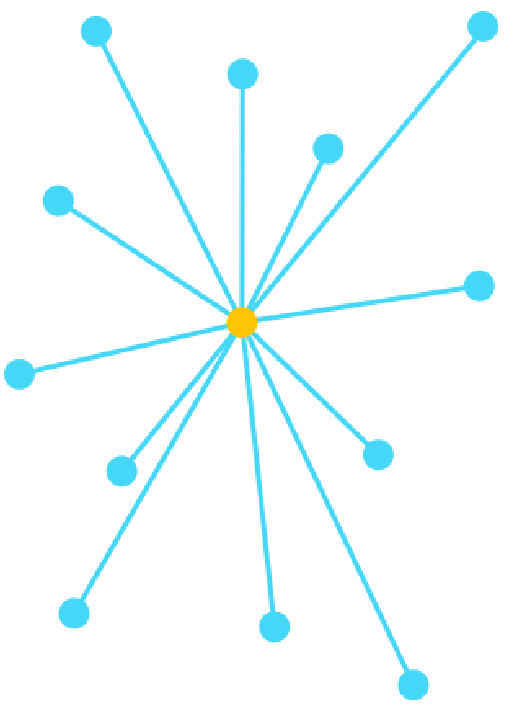
\includegraphics[width=0.4\textwidth,trim={0 0 0 0}]{figs/bootstrap_p2p.pdf}
        \centering
        \caption{Bootstrap}
    \end{subfigure}%
    \begin{subfigure}[t]{0.24\textwidth}
        \centering
        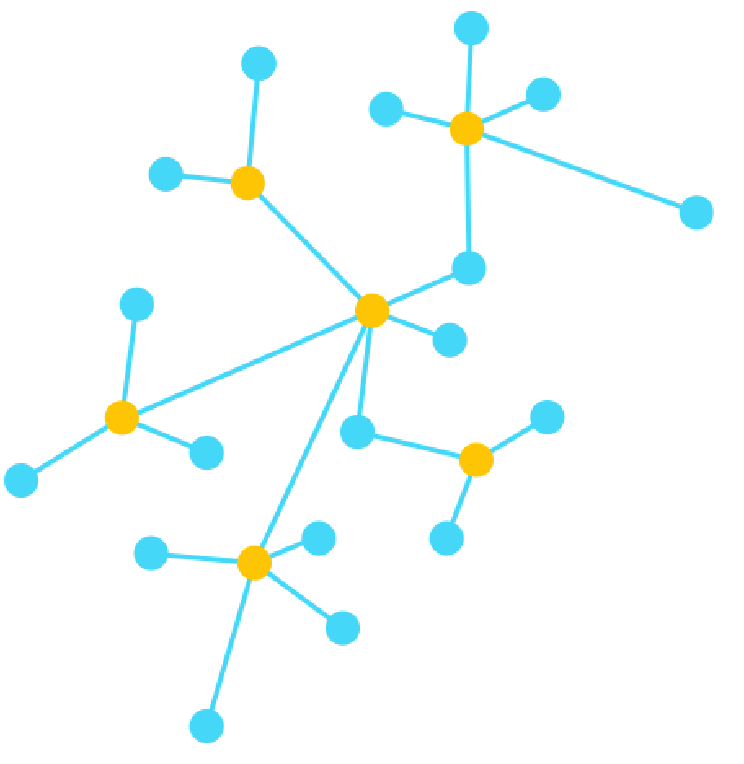
\includegraphics[width=0.5\textwidth,trim={0 0 0 0}]{figs/mdns_p2p.pdf}
        \centering
        \caption{mDNS}
    \end{subfigure}\\[1ex]
    \centering
    \begin{subfigure}[b]{0.4\textwidth}
        \centering
        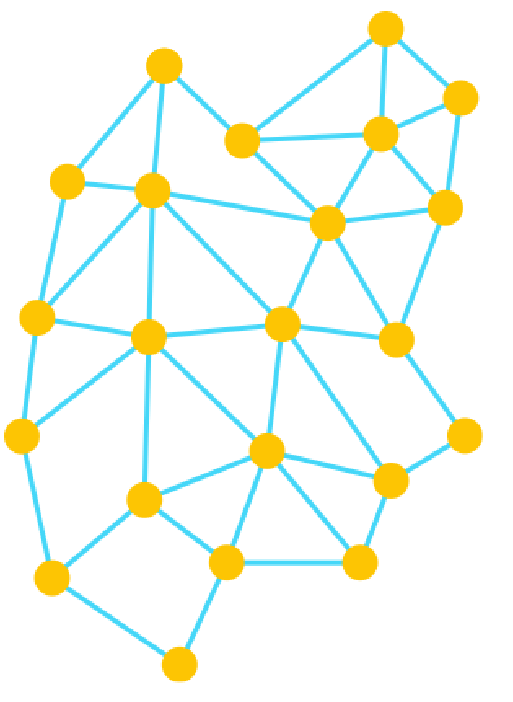
\includegraphics[width=0.25\textwidth,trim={0 0 0 0}]{figs/dht_p2p.pdf}
        \centering
        \caption{DHT Random Walk}
    \end{subfigure}
    \caption{Network structure after each peer discovery procedure}
    \label{fig:peer_discovery}
\end{figure}

\subsubsection{Peer Communication}
Vivian defines different libp2p protocols for different types of communications.
Messages are serialized via Protocol Buffers for better transmission performance.
For naming information updating among peers. We will going to implement Episub (similar to Gossip protocol) in libp2p pubsub protocols.
Considering the message redundancy issue, we plan to store the recently changed naming key-value pairs in cache for fast loop-up when handling gossip message from neighbors.

\subsection{Storage}
In this subsection we describe two potential implementations of file storage layer: via IPFS and via normal storage backends.

\subsubsection{IPFS}
IPFS is a decentralized peer-to-peer file system. When a file is uploaded to the system, it is split into many small blocks linked by a Merkle DAG.
The file and all of its blocks are given a unique hash fingerprint. The blocks of a file will be stored on different peers in the network in a distributed way.
Users can use the fingerprint of the file for content addressed searching for the file content.
The whole system is decentralized and files stored on the system are immutable. However, the fingerprint of a file is a cryptographic hash which is not human-meaningful.
Besides, traffic between nodes and content of the blocks are not encrypted and are visible to public.
In Vivian, if a user want to store his/her data via IPFS, he/she can first encrypt the file using GPG\footnote{GPG: GNU Privacy Guard. Open source alternative of Pretty Good Privacy (PGP)} and then upload to IPFS, then bind the fingerprint of the file to the name he/she owns.

\subsubsection{Normal Storage Backends}
Users can storage their data on normal storage Backends such as Amazon S3, Azure Blob and Google Cloud.
The intuitive idea is to split the file into small chunks encrypted and/or signed by user.
Then record the URI of these chunks on Tangle, and bind it to the name the user owns.
The message field of a Tangle transaction is 2,187 trytes in size and can sufficiently records a large number of URLs.
If the a single transaction is not enough to record all the URL, hierarchy tables can be implemented (similar to the idea of Bigtable by Google \cite{chang2008bigtable}).
In this way, the storage providers are only able to see the encrypted file chunks, and cannot parse the actual content of the files.